\section{Sensorik und Sicherheitstechnik \textcolor{gray}{(Elena Widmann)}}

\subsection{Aufgabenstellung}

\subsection{Sensorik}

\subsubsection{Endschalter}
Beim Verplanen der Endschalter ist zwischen Software- und Hardware-Endschalter zu unterscheiden. Die Software-Endschalter begrenzen den Arbeitsbereich der Achse und sollten innerhalb des Bereichs der Hardware-Endschalter parametriert werden. Ihre Positionen werden direkt im Siemens TIA-Portal eingestellt und können falls notwendig einfach auf die aktuelle Geschwindigkeit angepasst werden. Werden die Software-Endschalter angefahren, wird der Technologiealarm 533 ausgelöst, und die Dynamikwerte werden gestoppt, das Technologieobjekt bleibt hierbei freigegeben. Werden sie jedoch überfahren wird das Technologieobjekt gesperrt. \\
Die Hardware-Endschalter begrenzen den maximal zulässigen Verfahrensbereich der Achse. Bei ihnen wird nicht unterschieden, ob die Endschalter angefahren oder überfahren werden. Beim Anfahren der Schalter wird der Technologiealarm 531 ausgelöst. Er sperrt das Technologieobjekt und muss, bevor der Auslösebereich der Hardware-Endschalter wieder verlassen werden kann, quittiert werden. \cite{axis_manual}\\
Auf jeder der drei Achsen des AFSS, und auf dem Querförderer, müssen Hardware-Endschalter montiert werden. Die Auswahl begrenzte sich hierbei auf die uns zur Verfügung gestellten Sensoren, welche unter Berücksichtigung ihrer Funktion auf den verschiedenen Positionen eingebaut wurden.

\paragraph{Positionsschalter mit Rollhebel} \mbox{}\\
An der x-Achse werden als Hardware-Endschalter Positionsschalter mit Rollhebel verwendet (siehe Abb. \ref{roll_sens}). Von den insgesamt vier Stück werden zwei an der unteren und zwei an der oberen x-Achse befestigt. Davon besitzen drei jeweils einen Öffner- und einen Schließerkontakt \cite{schmersal_3}, wohingegen einer der Endschalter aus zwei Öffnerkontakten besteht \cite{schmersal_1}. Um Einheitlich zu bleiben, und da es sicherheitstechnisch auch von Vorteil ist (Drahtbruchsicherheit), verwenden wir jeweils einen der Öffnerkontakte der Endschalter. Zum Schalten des Rollhebels der Positionsschalter müssen auf dem x-Schlitten der oberen sowie unteren x-Achse Auslöser angebracht werden. Diese befinden sich mittig auf der Seite der Sensoren und gleichen einem vom Schlitten abstehenden Arm, welcher sich aus gestapelten, mit dem Lasercutter gefertigten, Teilen zusammensetzt.

\paragraph{Induktive Endschalter} \mbox{}\\
Als Hardware-Endschalter an der y-Achse werden induktive Sensoren verwendet (siehe Abb. \ref{ind_sens}). Davon werden zwei an der unteren und zwei an der oberen Seite der y-Achse befestigt, also auch hier wieder insgesamt vier Sensoren. Sie funktionieren so, dass durch eine Spule ein Magnetfeld erzeugt wird, welches dann in einem sich dem Sensor frontseitig nähernden elektrisch leitendem Material Wirbelströme erzeugt. Dadurch verändert sich das Magnetfeld und die Kontakte des induktive Sensors werden über einen Schmitt-Trigger geschaltet. Die Sensoren besitzen jeweils einen Öffner- und einen Schließerkontakt, wir verwenden jedoch ersteres um Drahtbruchsicherheit zu gewährleisten. Damit die induktiven Sensoren korrekt auslösen können, müssen auf dem Shuttle der y-Achse elektrisch leitende Gegenstücke angebracht werden.

\paragraph{Endtaster} \mbox{}\\
An der yz-Achse werden vier und am Querförderer zwei Stück mechanische Endtaster als Endschalter verwendet. Auf einem Endtaster befindet sich ein Schließerkontakt in Form eines Tasters, welcher durch anfahren geschalten wird (siehe Abb. \ref{tast_sens}). Zum Betätigen der Taster müssen sich Auslöser auf dem Shuttle und den Seiten der Querfördererstation befinden.\\

\begin{figure}[H]
    \centering
    \begin{subfigure}{.3\textwidth}
        \centering
        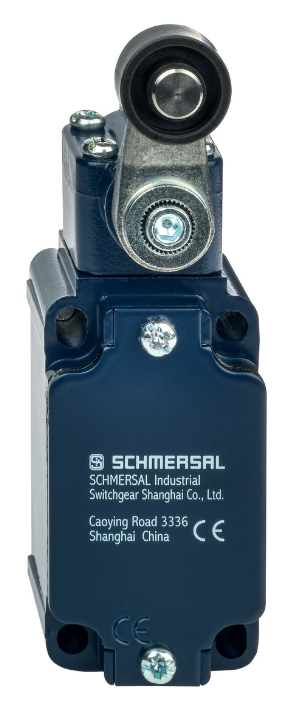
\includegraphics[width=0.5\textwidth]{Sensors/Rollendschalter.png}
        \caption{Rollendschalter \cite{schmersal_pic}}
        \label{roll_sens}
    \end{subfigure}%
    \begin{subfigure}{.3\textwidth}
        \centering
        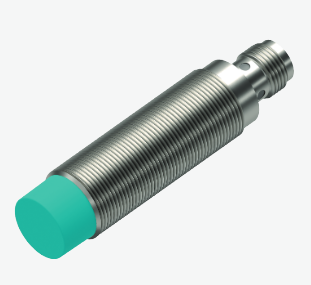
\includegraphics[width=1\textwidth]{Sensors/Induktiver_Sensor.png}
        \caption{Induktiver Sensor \cite{induktiv_sensor}}
        \label{ind_sens}
    \end{subfigure}%
    \begin{subfigure}{.3\textwidth}
        \centering
        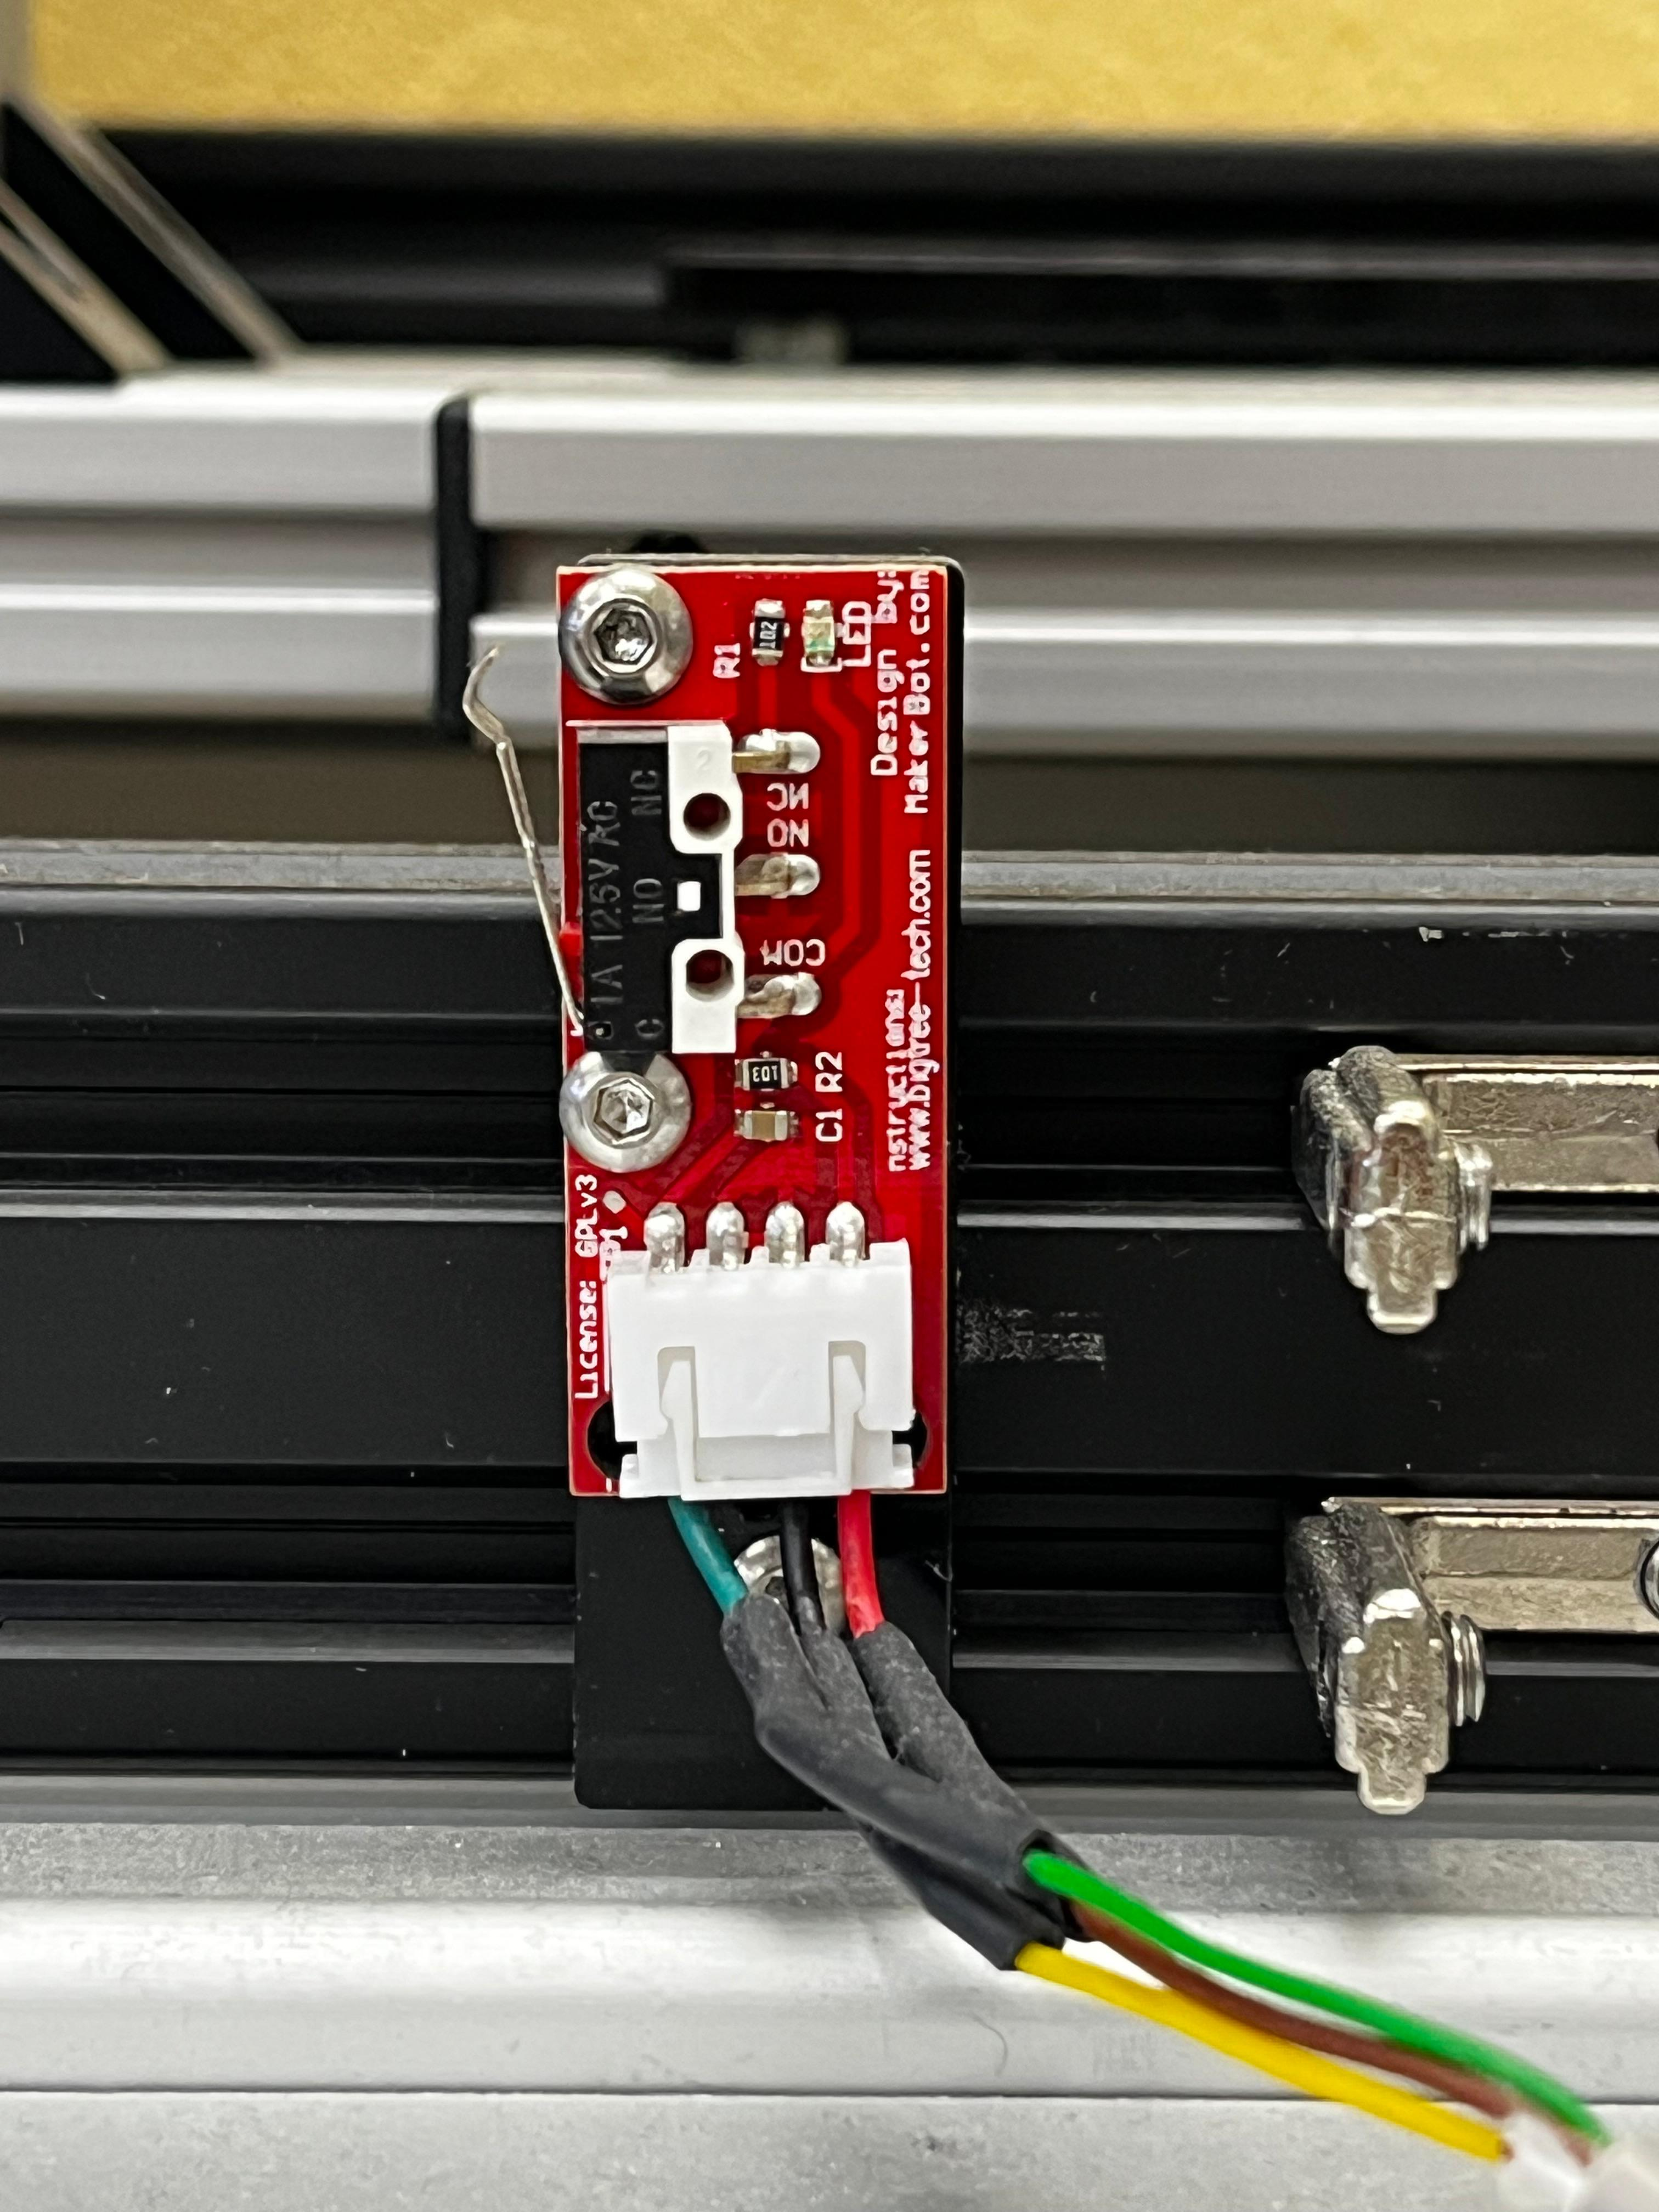
\includegraphics[width=0.9\textwidth]{Sensors/Endtaster.jpg}
        \caption{Endtaster}
        \label{tast_sens}
    \end{subfigure}
    \caption{Endschalter}
    \label{ulr}
\end{figure}

\subsubsection{Referenztaster}
Um die Motoren auf die richtige Position fahren zu können, müssen diese an allen drei Achsen und am Querförderer referenziert werden. Somit wird verhindert, dass bei einem Neustart des Systems sich die Koordinaten der Positionen, auf denen sich die Bauteilboxen befinden, nicht verändern und es zu keiner Kollision zwischen Shuttle und einer Box bzw. dem Gerüst kommt.\\
Zum Referenzieren müssen Sensoren an den Achsen und am Querförderer angebracht werden, welchen den jeweiligen Nullpunkt angeben. Hierfür werden Opto Interrupter verwendet, da diese einfach durch anfahren ausgelöst werden können. In einem Opto Interrupter befindet sich eine LED, dessen Lichtstrahl auf einen Photo Transistor trifft. Dieser schaltet daraufhin durch und es liegt eine Spannung am Emitter an. Wird jetzt jedoch der Lichtstrahl der LED unterbrochen, sperrt der Transistor und es fließt kein Strom. Bei der SPS-Programmierung ist daher zu beachten, dass sich der Ausgang des Sensors im nicht geschalteten Zustand auf HIGH befindet. Wird der Lichtstrahl jedoch unterbrochen, liegt am Sensorausgang keine Spannung an und der Eingang der SPS erhält ein LOW Signal.\\
Damit während eines Referenziervorgangs der Lichtstrahl der LED unterbrochen wird und der Referenztaster auslöst, müssen auch hier wieder Auslösevorrichtungen an den beiden x-Schlitten, am Shuttle und an der Querfördererstation angebracht werden.\\
In unserem Fall werden TP808 zum Referenzieren verwendet. Hierbei ist zu beachten, dass die sich darin befindende Diode nur mit einer maximalen Flussspannung von \qty{1.35}{\volt} betrieben werden darf.\cite{TP808} Da die Opto Interrupter jedoch über ASi-Bus mit der SPS verbunden werden, welche eine Spannung von \qty{24}{\volt} liefert, musste eine eigene Platine entworfen und gelötet werden, um das Bauteil nicht mit einer zu hohen Betriebsspannung zu zerstören. Hierfür wurde die Software Fusion360 verwendet, welche das Designen von Leiterplatten ermöglicht. Hergestellt wurden diese dann durch unsere eigene schulinterne Leiterplattenfertigung. Insgesamt musste die Referenzplatine sieben mal hergestellt werden.

\paragraph{Schaltungsentwurf} \mbox{}\\
Die Schaltung sollte so konzipiert werden, dass keines der involvierten Bauteile über längeren Normalbetrieb oder durch kurzzeitige hohe Ströme bzw. Spannungen, beschädigt wird. Das Ziel ist, die korrekte Funktion des Opto Interrupters auch zukünftig noch sicher stellen zu können. Dafür ist besonders wichtig auf dessen elektrische Eigenschaften zu achten, welche im Datenblatt zu finden sind. Für den fertigen Entwurf der Schaltung siehe Abb.\ref{Ref_Schaltplan}\\
Im Opto Interrupter befindet sich eine LED mit einer maximalen Durchlassspannung von \qty{1.35}{\volt}. und einer typischen Durchlassspannung V$_{F}$ von \qty{1.2}{\volt}. Um diese nicht mit den vollen \qty{24}{\volt} der Betriebsspannung V$_{B}$ zu überlasten muss ein Vorwiderstand R$_{1}$ eingebaut werden. Um die LED zum leuchten zu bringen, soll ein minimaler I$_{F}$ von \qty{10}{\milli\ampere} fließen. Dann lässt sich daraus der Vorwiderstand aus dem ohmschen Gesetz und mit Hilfe der Maschenregel berechnen:

\begin{equation*}
    R_{1} = \frac{V_{B} - V_{F}}{I_{F}} = \frac{\qty{24}{\volt} - \qty{1.2}{\volt}}{\qty{10}{\milli\ampere}} = \qty{2.28}{\kilo\ohm}
\end{equation*}

In der HTL wir den Schülerinnen und Schülern die Widerstandsreihe E12 zur Verfügung gestellt. Daher wird in der Schaltung der nächstgrößere Widerstand mit dem Wert $\qty{2,7}{\kilo\ohm}$ verwendet.\\
Der Phototransistor, welcher als Gegenstück zur LED dient, darf mit einer maximalen Collector-Emitter-Spannung von \qty{30}{\volt} betrieben werden, wodurch er gut geeignet ist für das Ziel der Schaltung. Um jedoch im besten Fall die gesamten \qty{24}{\volt} für den Eingang der SPS an der Klemme X1 abgreifen zu können, wird ein Spannungsteiler verwendet, bei dem nach dem Transistor ein Widerstand R$_{3}$ parallel zur Klemme X1 eingebaut wird. Da nur ein niedriger Strom benötigt wird, kann I$_{R3}$ relativ klein sein, hier \qty{1}{\milli\ampere}. Daraus lässt sich dann der Widerstandswert wie folgt berechnen:

\begin{equation*}
    R_{3} = \frac{V_{B}}{I_{R3}} = \frac{\qty{24}{\volt}}{\qty{1}{\milli\ampere}} = \qty{24}{\kilo\ohm}
\end{equation*}

Auch hier wird wieder der nächstgrößere Widerstandswert, der zur Verfügung gestellt wird, verwendet. R$_{3}$ entspricht somit dem Wert $\qty{27}{\kilo\ohm}$.\\
Für Funktionstests und die Inbetriebnahme ist es wichtig, dass eine Möglichkeit gegeben ist, den Zustand des Ausgangs der Schaltung anzuzeigen. Hierfür wird eine grüne 5mm LED verwendet, welche parallel zur Klemme X1 eingebaut wird. Da der Transistor einen maximalen Collector Strom von \qty{20}{\milli\ampere} besitzt, wurde die Entscheidung getroffen, die grüne LED nur mit \qty{10}{\milli\ampere} zu versorgen, da diese auch bei geringerem Strom genug Leuchtkraft für den benötigten Zweck besitzt. Bei einem Strom I$_{R2}$ von \qty{10}{\milli\ampere} besitzt die LED einen Spannungsabfall V$_{LED}$ von \qty{2.1}{\volt}.\cite{led_grün} Daraus lässt sich dann er Widerstand R$_{2}$ berechnen:

\begin{equation*}
    R_{2} = \frac{V_{B} - V_{LED}}{I_{R2}} = \frac{\qty{24}{\volt} - \qty{2.1}{\volt}}{\qty{10}{\milli\ampere}} = \qty{2.19}{\kilo\ohm}
\end{equation*}

Der nächsthöhere Widerstand der E12 Reihe entspricht $\qty{2,2}{\kilo\ohm}$, um auf Nummer sicher zu gehen wird jedoch der um eine Stufe größere Widerstand mit einem Wert von $\qty{2,7}{\kilo\ohm}$ verwendet. Wenn der Lichtstrahl im Opto Interrupter nicht unterbrochen wird und der Transistor somit durchschaltet, leuchtet die grüne LED. Wird jetzt der Lichtstrahl unterbrochen erlischt die LED. Damit diese nicht während des Normalbetriebs dauerhaft leuchtet wird ein Jumper eingebaut, mit welchen die LED ganz einfach aus der Schaltung ausgeschlossen werden kann.

\begin{figure}[H]
    \centering
    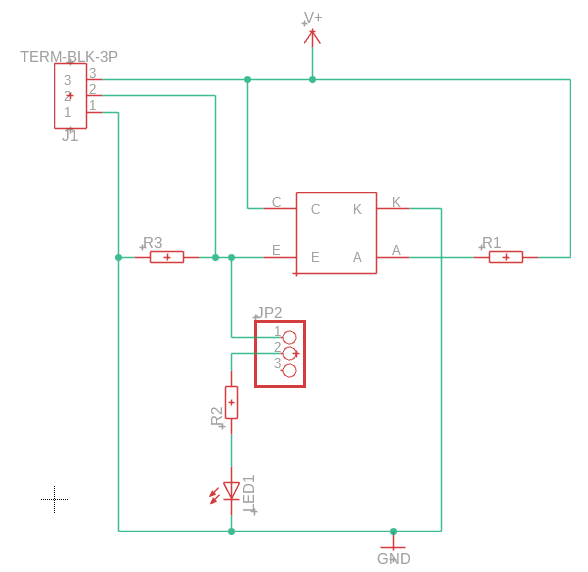
\includegraphics[width=0.6\textwidth]{Sensors/Ref_Schaltplan.png}
    \caption{Schaltplan Referenzplatine}
    \label{Ref_Schaltplan}
\end{figure}

\paragraph{Platinenentwurf und -herstellung} \mbox{}\\
Um die benötigten Referenzplatinen herstellen zu können, muss zuerst ein Leiterplattenplan in Fusion360, ehemals Eagle, erstellt werden. Über den Sharepoint der HTL lässt sich eine Elektronikbibliothek, die alle in der Schule verfügbaren Bauteile beinhaltet, herunterladen. Da der in der Schaltung verwendete Opto Interrupter nicht in der Schule verfügbar ist, sondern extern organisiert werden musst, befindet er sich nicht in dieser Elektronikbibliothek. Daher muss für ihn ein eigenes Symbol sowie ein dazugehöriger Footprint gezeichnet werden.\\
Zum Entwerfen des Printed Circuit Boards (PCB) muss ein neuer Elektronikentwurf in Fusion erstellt werden. Hier muss zuerst der zugehörige Schaltplan gezeichnet werden. Wichtig ist, dass bei der dreipoligen Schraubklemme das Bauteil 3282837-3 (J1) verwendet wird, da sonst die Abstände zwischen den Lötpads zu klein und diese zu nah bei einander sind. Damit der Jumper (JP2) nicht verloren geht, wenn die Verbindung zwischen Ground und LED aufgehoben werden soll, wird ein dreipoliger Pinheader verwendet, um den Jumper für den gegebenen Zeitraum einfach umstecken zu können.\\
Nach Fertigstellung des Schaltplans kann in Fusion ein passendes Leiterplattendokument erstellt werden, welches die Bauteile und die zugehörigen Verbindungen direkt übernimmt. Für den fertigen Leiterplattenplan des Referenztasters siehe Abb.\ref{Ref_LPPlan}. Da beim verwendeten Opto Interrupter Löcher zur Montierung vorhanden sind, müssen auf der Platine selbst keine zusätzlichen Bohrungen eingeplant werden. Bein der Anordnung der Bauteile auf der Platine ist zu beachten, dass sich die Löcher am Opto Interrupter, am schmäleren rand der Platine befinden. Um eine leichtere Verkabelung zu ermöglichen, sollte auch die Schraubklemme am Rand der Platine platziert werden.

\begin{figure}[H]
    \centering
    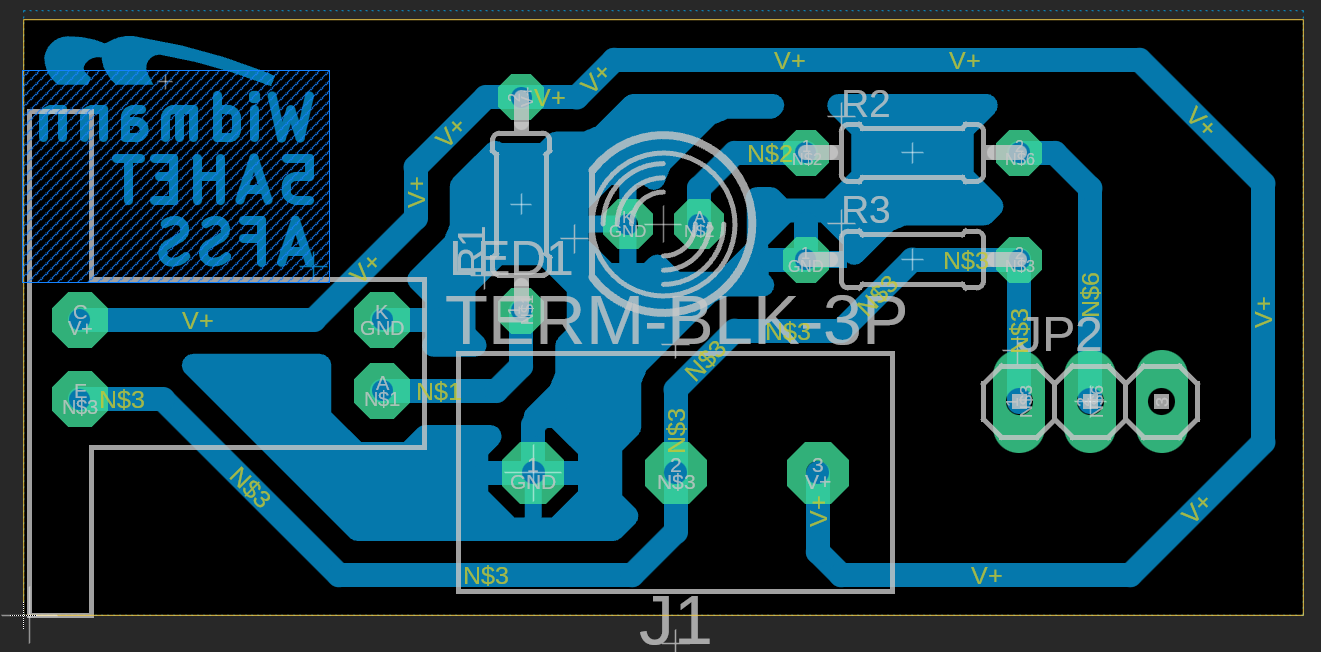
\includegraphics[width=0.7\textwidth]{Sensors/Ref_Leiterplattenplan.png}
    \caption{Leiterplattenplan Referenzplatine}
    \label{Ref_LPPlan}
\end{figure}

Wenn die Bauteile alle platziert und verbunden worden sind, sowie ein Polygon über die gesamte Platine gezogen worden ist, muss diese noch auf Fehler geprüft werden. Auch hier ist eine bereits fertige Datei, welche die benötigten Design Rules für Fusion360 beinhaltet, auf der Schulwebsite zu finden. Wichtig ist, damit die Platine zur Produktion in der Leiterplattenfertigung der HTL eingereicht werden kann, muss diese den vorgegebenen Anforderungen entsprechen. Dazu gehört, dass sich das HTL-Logo auf der Platine befindet und die Texteinstellungen Font: Vector, Ratio: \qty{16}{\percent} und Size: min \qty{70}{mil} entsprechen. Auch die Breite der Kupferbahnen darf nicht zu klein sein (hier: \qty{32}{mil}).\\
Nach Einreichung des Fertigungsauftrags wird die Platine von Schülerinnen und Schülern der HTL gefertigt. Der Prozess startet mit dem Reinigen des Basismaterials, um es daraufhin mit dem Negativtrockenresist (Trockenfilm) zu laminieren. In den nächsten Schritten werden die Layout-Informationen mit einem Belichter auf das Laminat übertragen und das unbelichtete Laminat mit einer Natrium-Carbonat Lösung von der Platine entfernt. Daraufhin werden durch Ätzen mit einer Eisen-III-Chlorid-Lösung strukturierte Kupferflächen freigestellt. Als Nächstes werden die Löcher in die Kupferpads gebohrt und die Platine auf ihre korrekte Größe zugeschnitten. Durch das Legen der Leiterplatte in eine Entschichtlösung aus \qty{5}{\percent}{igem} Kaliumcarbonat mit Wasser werden Ätzresiste von der Platine entfernt. Zu guter Letzt wird die Platine mit einem Versiegelungslack versiegelt, um sie vor Umwelteinflüssen und Korrosion zu schützen.

\paragraph{Platinentestung und Messung} \mbox{}\\
Um die korrekte Funktionsweise der Referenzplatine sicher zu stellen, muss diese nach dem Löten getestet werden. An der Klemme X1 wurden Spannungswerte zwischen \qtyrange{19.7}{21.3}{\volt} gemessen. Obwohl die Spannungen unter den gewünschten \qty{24}{\volt} liegen können die Platinen problemlos verwendet werden, da die verwendeten AS-i-Slaves einen minimalen HIGH-Eingangsschaltpegel von \qty{10}{\volt} besitzen.\cite{AS-i-Slave}

\subsubsection{Lichttaster}

\subsubsection{Barcode-Scanner}
\begin{wrapfigure}{R}{0.34\textwidth}
    \vspace{-20px}
    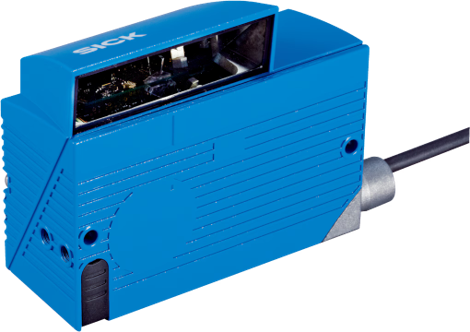
\includegraphics[width=0.34\textwidth]{Sensors/Barcodescanner.png}
    \caption{Barcodescanner CLV61x-2Port}
    \label{BarScan}
\end{wrapfigure}

Durch anbringen eines sich nicht wiederholenden Barcodes auf jeder Box wird eine gute Möglichkeit geschaffen, in der Software den Behälter und die sich darin befindenden Bauteile einander zuzuordnen. Unter der Voraussetzung, dass die Benutzerinnen und Benutzer vor jeder Wiedereinlagerung ihrer Box zuerst dessen Barcode einscannen, wird die Wahrscheinlichkeit, dass der Lagerplatz einer Box falsch abgespeichert wird, verkleinert. Somit sinkt die Chance, dass bei Bestellen eines Bauteils die falsche Komponente geliefert wird. Das erfassen des Barcodes findet mittels eines Barcodescanners der Firma SICK statt (siehe Abb.\ref{BarScan}), welcher bei der Kommissionierstation untergebracht ist, um eine einfache Bedienung gewährleisten zu können.\\
Der uns zur Verfügung gestellte Barcodescanner (CLV61x-2Port) ist in der Lage alle gängigen Codearten einzulesen.\cite{Barcodescanner} Barcodes wurden so entwickelt, dass bereits beim Einlesen erkannt wird, wo dieser anfängt und aufhört, damit beim einscannen nicht auf die richtige Ausrichtung geachtet werden muss.

\paragraph{Einbindung ins TIA-Portal \cite{BarScan_Handbuch}}\mbox{}\\
Damit der eingelesene Barcode an den Webserver weitergegeben werden kann, muss dieser im Siemens TIA-Portal abgespeichert werden. Mit der CPU verbunden wird der Scanner über PROFINET. Hierbei handelt es sich um einen auf Industrial Ethernet basierenden Kommunikationsstandard und eine Weiterentwicklung des PROFIBUS Vorgängers. Über ihn lässt sich die gescannte Nummer ganz einfach an die SPS übermitteln.\\
Im TIA-Portal Projekt muss, um eine Verbindung zum Barcodescanner herstellen zu können, die zugehörige Gerätebeschreibungsdatei (GSD-Datei) installiert werden. Dies funktioniert über das Gerätebeschreibungsdateien verwalten Fenster im TIA-Portal. Nach der Installation ist das Gerät im Hardwarekatalog unter \enquote{Weitere Feldgeräte} zu finden. Die benötigte Datei wird auf der Internetseite des Herstellers als Download zur Verfügung gestellt.

\paragraph{Auslesen des Barcodes}\mbox{}\\
Wenn eine Verbindung zum Gerät hergestellt wurde, müssen die Parametermodule eingefügt und richtig eingestellt werden. Diese werden über den Hardware-Katalog ausgewählt und eingefügt, für eine Übersicht der eingefügten Module siehe Abb.\ref{BarScan_TIA}. Wichtig ist, bei den Baugruppenparametereinstellungen von \enquote{\mbox{47\_Communication Mode\_1}} \enquote{No Handshake} auszuwählen und bei \enquote{\mbox{99\_End Remote Config}}
\enquote{Don't save parameters perm.} einzustellen. Um die verwendeten Art von Barcodes einscannen zu können muss darauf geachtet werden, dass er unter \enquote{\mbox{22\_UPC EAN GTIN\_1}} ausgewählt und somit eingeschaltet ist.\\

\begin{figure}[h]
    \centering
    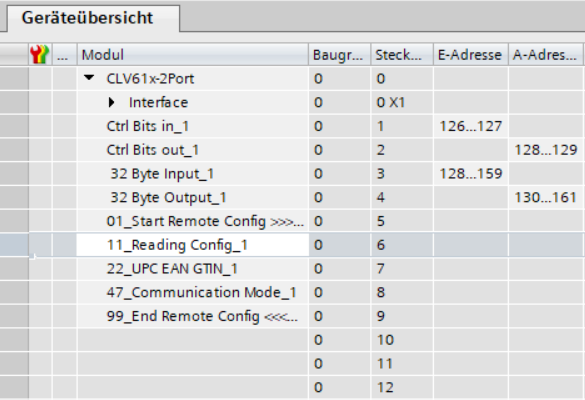
\includegraphics[width=0.6\textwidth]{Sensors/BarScan_Geräteübersicht.png}
    \caption{Barcodescanner Geräteübersicht im TIA-Portal\cite{BarScan_pic}}
    \label{BarScan_TIA}
\end{figure}

Die vom Barcodescanner belegten Ein- und Ausgangsadressen sind in der Geräteübersicht ersichtlich (siehe Abb.\ref{BarScan_TIA}). Ein TriggerBit wird verwendet um das Einlesen eines Barcodes zu starten, dabei handelt es sich um das zweite Bit des \enquote{\mbox{Ctrl Bits out\_1}} Moduls (hier: Q129.0). Bei steigender Flanke des ToggleBits wird der Laser eingeschaltet, erst bei der fallenden Flanke wird daraufhin der Code eingelesen.\\
Die eingelesenen Daten liegen ab dem ersten Input Byte (hier: ab IB128.0). Auf dem ersten Input Byte wird am vierten Bit ein ToggleBit mitgeführt. Am zweiten Byte(IB129.0) befindet sich ein Zähler, der mitzählt, wie viele Codes bereits eingelesen wurden. Das vierte Input Byte (IB131.0) gibt die Länge des eingelesenen Strings an. Ab dem sechsten Byte (IB133.0) stehen die eigentlichen Daten des Barcodes.\\
Um die Daten des Barcodes überprüfen zu können eignet sich eine wie in Abb.\ref{} abgebildete Beobachtungstabelle. Wichtig ist, dass beim Einfügen der Ein- und Ausgangsadressen das richtige Zeichenformat ausgewählt wird. Um eine Überprüfung durchzuführen lässt sich das ToggleBit zum Starten es Einlesevorgangs über Eingabe von TRUE und FALSE setzen, und daraufhin ein Code scannen. Die einzelnen Input Bytes werden daraufhin in der Tabelle angezeigt. \textbf{Foto einfügen!!}

\subsection{AS-Interface}

\subsubsection{Allgemeines}

\subsubsection{Programmierung im TIA-Portal}

\subsubsection{Verkabelung}


\subsection{Sicherheitstechnik}
\subsubsection{Grundanforderungen und Planung}
\subsubsection{Realisierung}